\begin{task}
Wyznacz współczynniki trygonometrzycznego szeregu fouriera dla okresowego sygnału $f(t)$ przedstawionego na rysunku 

\begin{figure}[H]
\centering
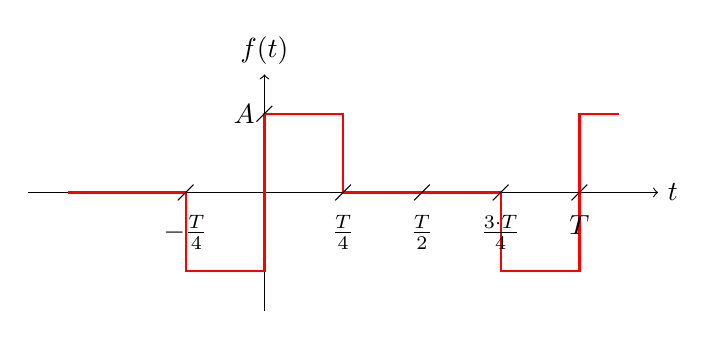
\begin{tikzpicture}
  %\draw (0,0) circle (1in);
  \draw[->] (-3.0,+0.0) -- (+5.0,+0.0) node[right] {$t$};
  \draw[->] (+0.0,-1.5) -- (+0.0,+1.5) node[above] {$f(t)$};
  \draw[-,red, thick] (-2.5,+0.0) -- (-1.0,+0.0) -- (-1.0,-1.0)--(+0.0,-1.0) -- (+0.0,+1.0) -- (+1.0,+1.0) -- (+1.0,+0.0) -- (+3.0,+0.0) -- (+3.0,-1.0) -- (4.0,-1.0) -- (4.0,1.0) -- (4.5,1.0);
  %\draw[-] (-1.0-0.1,-0.1)--(-1.0+0.1,0.1) node[midway, below, outer sep=10pt,align=center] {$-\frac{T}{2}$};
  \draw[-] (-1.0-0.1,-0.1)--(-1.0+0.1,0.1) node[midway, below, outer sep=5pt,align=center] {$-\frac{T}{4}$};
  \draw[-] (+1.0-0.1,-0.1)--(+1.0+0.1,0.1) node[midway, below, outer sep=5pt] {$\frac{T}{4}$};
  \draw[-] (+2.0-0.1,-0.1)--(+2.0+0.1,0.1) node[midway, below, outer sep=5pt] {$\frac{T}{2}$};
  \draw[-] (+3.0-0.1,-0.1)--(+3.0+0.1,0.1) node[midway, below, outer sep=5pt] {$\frac{3\cdot T}{4}$};
  \draw[-] (+4.0-0.1,-0.1)--(+4.0+0.1,0.1) node[midway, below, outer sep=5pt] {$T$};
  \draw[-] (-0.1,1.0-0.1)--(+0.1,1.0+0.1) node[midway, left] {$A$};
\end{tikzpicture}
\end{figure}

W pierwszej kolejności należy opisać sygnał za pomocą wzoru.

\begin{equation}
   f(x)=\begin{cases}-A & t \in \left (  -\frac{T}{4}+k \cdot T; 0+k \cdot T \right ) \\A & t \in \left (  0+k \cdot T; \frac{T}{4}+k \cdot T \right ) \\0 & t \in \left ( \frac{T}{4}+k \cdot T; \frac{3\cdot T}{4} +k \cdot T\right )\end{cases} \wedge k \in C %\mathbb{C}
\end{equation}

Współczynnik $a_0$ wyznaczamy ze wzoru

\begin{equation}
a_0=\frac{1}{T}\int_{T}f(t) \cdot dt
\end{equation}

Podstawiamy do wzoru wzór naszej funkcji w pierwszym okresie $k=0$

\begin{align*}
a_0 &=\frac{1}{T}\int_{T}f(t) \cdot dt =\\
&=\frac{1}{T} \left( \int_{-\frac{T}{4}}^{0} -A \cdot dt + 
\int_{0}^{\frac{T}{4}} A \cdot dt +
\int_{\frac{T}{4}}^{\frac{3\cdot T}{4}} 0 \cdot dt \right ) = \\
&=\frac{1}{T} \left( \int_{-\frac{T}{4}}^{0} -A \cdot dt + 
\int_{0}^{\frac{T}{4}} A \cdot dt + 0 \right ) = \\
&=\frac{1}{T} \left( -A \cdot \int_{-\frac{T}{4}}^{0} dt + 
A \cdot \int_{0}^{\frac{T}{4}} dt + 0 \right ) = \\
&=\frac{1}{T} \left( -A \cdot \left. t \right|_{-\frac{T}{4}}^{0} + 
A \cdot \left. t \right|_{0}^{\frac{T}{4}}\right ) = \\
&=\frac{1}{T} \left( -A \cdot \left( 0 - \left(-\frac{T}{4}\right) \right) + 
A \cdot \left( \frac{T}{4} - 0 \right)\right ) = \\
&=\frac{1}{T} \left( -A \cdot \frac{T}{4} + 
A \cdot \frac{T}{4}\right ) = \\
&=\frac{1}{T} \left( 0 \right ) = \\
&=0
\end{align*}

Wartość współczynnika $a_0$ wynosi $0$


Współczynnik $a_k$ wyznaczamy ze wzoru

\begin{equation}
a_k=\frac{2}{T}\int_{T}f(t) \cdot cos\left( k \cdot \frac{2\pi}{T} \cdot t\right) \cdot dt
\end{equation}

Podstawiamy do wzoru wzór naszej funkcji w pierwszym okresie $k=0$

\begin{align*}
a_k&=\frac{2}{T}\int_{T}f(t) \cdot cos\left( k \cdot \frac{2\pi}{T} \cdot t\right) \cdot dt=\\
&=\frac{2}{T}\left(\int_{-\frac{T}{4}}^{0} -A \cdot cos\left( k \cdot \frac{2\pi}{T} \cdot t\right) \cdot dt 
+ \int_{0}^{\frac{T}{4}} A \cdot cos\left( k \cdot \frac{2\pi}{T} \cdot t\right) \cdot dt
+ \int_{\frac{T}{4}}^{\frac{3\cdot T}{4}} 0 \cdot cos\left( k \cdot \frac{2\pi}{T} \cdot t\right) \cdot dt \right)=\\
&=\frac{2}{T}\left(-A \cdot \int_{-\frac{T}{4}}^{0} cos\left( k \cdot \frac{2\pi}{T} \cdot t\right) \cdot dt 
+ A \cdot \int_{0}^{\frac{T}{4}} cos\left( k \cdot \frac{2\pi}{T} \cdot t\right) \cdot dt
+ \int_{\frac{T}{4}}^{\frac{3\cdot T}{4}} 0 \cdot dt \right)=\\
&=\begin{Bmatrix*}[l]
z&=k \cdot \frac{2\pi}{T} \cdot t \\
dz&=k \cdot \frac{2\pi}{T} \cdot dt \\
dt&=\frac{dt}{k \cdot \frac{2\pi}{T}}
\end{Bmatrix*} =\\
&=\frac{2}{T}\left(-A \cdot \int_{-\frac{T}{4}}^{0} cos\left( z \right) \cdot \frac{dt}{k \cdot \frac{2\pi}{T}} 
+ A \cdot \int_{0}^{\frac{T}{4}} cos\left( z \right) \cdot \frac{dt}{k \cdot \frac{2\pi}{T}}
+ 0 \right)=\\
&=\frac{2}{T}\left(-\frac{A}{k \cdot \frac{2\pi}{T}} \cdot \int_{-\frac{T}{4}}^{0} cos\left( z \right) \cdot dt 
+ \frac{A}{k \cdot \frac{2\pi}{T}} \cdot \int_{0}^{\frac{T}{4}} cos\left( z \right) \cdot dt\right)=\\
&=\frac{2}{T} \cdot \frac{A}{k \cdot \frac{2\pi}{T}} \cdot \left(- \left. sin\left( z \right) \right|_{-\frac{T}{4}}^{0}
+ \left. sin\left( z \right)\right|_{0}^{\frac{T}{4}} \right)=\\
&=\frac{2 \cdot A}{k \cdot 2\pi} \cdot \left(- \left. sin\left( k \cdot \frac{2\pi}{T} \cdot t  \right) \right|_{-\frac{T}{4}}^{0}
+ \left. sin\left( k \cdot \frac{2\pi}{T} \cdot t  \right)\right|_{0}^{\frac{T}{4}} \right)=\\
&=\frac{2 \cdot A}{k \cdot 2\pi} \cdot \left(- \left( sin\left( k \cdot \frac{2\pi}{T} \cdot 0  \right) - sin\left( - k \cdot \frac{2\pi}{T} \cdot \frac{T}{4}  \right) \right)
+ \left( sin\left( k \cdot \frac{2\pi}{T} \cdot \frac{T}{4}  \right) - sin\left( k \cdot \frac{2\pi}{T} \cdot 0  \right)\right) \right)=\\
&=\frac{A}{k \cdot \pi} \cdot \left(- \left( sin\left( 0 \right) - sin\left( - k \cdot \frac{2\pi}{4} \right) \right)
+ \left( sin\left( k \cdot \frac{2\pi}{4} \right) - sin\left( 0 \right)\right) \right)=\\
&=\frac{A}{k \cdot \pi} \cdot \left(- \left( 0 - sin\left( - k \cdot \frac{\pi}{2} \right) \right)
+ \left( sin\left( k \cdot \frac{\pi}{2} \right) - 0\right) \right)=\\
&=\frac{A}{k \cdot \pi} \cdot \left(sin\left( - k \cdot \frac{\pi}{2} \right)
+ sin\left( k \cdot \frac{\pi}{2} \right) \right)=\\
&=\frac{A}{k \cdot \pi} \cdot \left(- sin\left( k \cdot \frac{\pi}{2} \right)
+ sin\left( k \cdot \frac{\pi}{2} \right) \right)=\\
&=\frac{A}{k \cdot \pi} \cdot \left(0 \right)=\\
&=0
\end{align*}

Wartość współczynnika $a_k$ wynosi $0$


Współczynnik $b_k$ wyznaczamy ze wzoru

\begin{equation}
b_k=\frac{2}{T}\int_{T}f(t) \cdot sin\left( k \cdot \frac{2\pi}{T} \cdot t\right) \cdot dt
\end{equation}

Podstawiamy do wzoru wzór naszej funkcji w pierwszym okresie $k=0$

\begin{align*}
b_k&=\frac{2}{T}\int_{T}f(t) \cdot sin\left( k \cdot \frac{2\pi}{T} \cdot t\right) \cdot dt=\\
&=\frac{2}{T} \left(\int_{-\frac{T}{4}}^{0}-A \cdot sin\left( k \cdot \frac{2\pi}{T} \cdot t\right) \cdot dt 
+ \int_{0}^{\frac{T}{4}} A \cdot sin\left( k \cdot \frac{2\pi}{T} \cdot t\right) \cdot dt 
+ \int_{\frac{T}{4}}^{\frac{3\cdot T}{4}} 0 \cdot sin\left( k \cdot \frac{2\pi}{T} \cdot t\right) \cdot dt \right)=\\
&=\frac{2}{T} \left(-A \cdot \int_{-\frac{T}{4}}^{0} sin\left( k \cdot \frac{2\pi}{T} \cdot t\right) \cdot dt 
+  A \cdot \int_{0}^{\frac{T}{4}} sin\left( k \cdot \frac{2\pi}{T} \cdot t\right) \cdot dt 
+ \int_{\frac{T}{4}}^{\frac{3\cdot T}{4}} 0 \cdot dt \right)=\\
&=\begin{Bmatrix*}[l]
z&=k \cdot \frac{2\pi}{T} \cdot t \\
dz&=k \cdot \frac{2\pi}{T} \cdot dt \\
dt&=\frac{dz}{k \cdot \frac{2\pi}{T}} \\
\end{Bmatrix*}=\\
&=\frac{2}{T} \left(-A \cdot \int_{-\frac{T}{4}}^{0} sin\left( z \right) \cdot \frac{dz}{k \cdot \frac{2\pi}{T}}  
+  A \cdot \int_{0}^{\frac{T}{4}} sin\left( z \right) \cdot \frac{dz}{k \cdot \frac{2\pi}{T}}  
+ 0 \right)=\\
&=\frac{2}{T} \left(-\frac{A}{k \cdot \frac{2\pi}{T}} \cdot \int_{-\frac{T}{4}}^{0} sin\left( z \right) \cdot dz  
+  \frac{A}{k \cdot \frac{2\pi}{T}} \cdot \int_{0}^{\frac{T}{4}} sin\left( z \right) \cdot dz \right)=\\
&=\frac{2}{T} \cdot \frac{A}{k \cdot \frac{2\pi}{T}} \cdot \left(- \int_{-\frac{T}{4}}^{0} sin\left( z \right) \cdot dz  
+  \int_{0}^{\frac{T}{4}} sin\left( z \right) \cdot dz \right)=\\
&=\frac{A}{k \cdot \pi} \cdot \left(\left. cos\left( z \right) \right|_{-\frac{T}{4}}^{0} - \left. cos\left( z \right) \right|_{0}^{\frac{T}{4}} \right)=\\
&=\frac{A}{k \cdot \pi} \cdot \left(\left. cos\left( k \cdot \frac{2\pi}{T} \cdot t \right) \right|_{-\frac{T}{4}}^{0} - \left. cos\left( k \cdot \frac{2\pi}{T} \cdot t \right) \right|_{0}^{\frac{T}{4}} \right)=\\
&=\frac{A}{k \cdot \pi} \cdot \left(\left( cos\left( k \cdot \frac{2\pi}{T} \cdot 0 \right) - cos\left(- k \cdot \frac{2\pi}{T} \cdot \frac{T}{4} \right) \right) - \left( cos\left( k \cdot \frac{2\pi}{T} \cdot \frac{T}{4} \right) - cos\left( k \cdot \frac{2\pi}{T} \cdot 0 \right) \right) \right)=\\
&=\frac{A}{k \cdot \pi} \cdot \left(\left( cos\left(0 \right) - cos\left(- k \cdot \frac{\pi}{2} \right) \right) - \left( cos\left( k \cdot \frac{\pi}{2} \right) - cos\left( 0 \right) \right) \right)=\\
&=\frac{A}{k \cdot \pi} \cdot \left( cos\left(0 \right) - cos\left(- k \cdot \frac{\pi}{2} \right) - cos\left( k \cdot \frac{\pi}{2} \right) + cos\left( 0 \right) \right)=\\
&=\frac{A}{k \cdot \pi} \cdot \left( 1 - cos\left( k \cdot \frac{\pi}{2} \right) - cos\left( k \cdot \frac{\pi}{2} \right) + 1 \right)=\\
&=\frac{A}{k \cdot \pi} \cdot \left( 2 - 2 \cdot cos\left(k \cdot \frac{\pi}{2} \right) \right)=\\
&=\frac{2 \cdot A}{k \cdot \pi} \cdot \left( 1 - cos\left(k \cdot \frac{\pi}{2} \right) \right)
\end{align*}

Wartość współczynnika $b_k$ wynosi $\frac{2 \cdot A}{k \cdot \pi} \cdot \left( 1 - cos\left(k \cdot \frac{\pi}{2} \right) \right)$


Ostatecznie współczynniki trygonometrycznego szeregu fouriera dla funkcji przedstawionej na rysunku przyjmują wartości

\begin{align*}
a_0&=0\\
a_k&=0\\
b_k&=\frac{2 \cdot A}{k \cdot \pi} \cdot \left( 1 - cos\left(k \cdot \frac{\pi}{2} \right) \right)\\
\end{align*}

Możemy wyznaczyć kilka wartości współczynników $a_k$ i $b_k$

\begin{table}[H]
\centering  
\begin{tabular}{|c|c|c|c|c|c|c|}
  \hline 
  $k$ & $1$ & $2$ & $3$ & $4$ & $5$ & $6$\\ 
  \hline 
  $a_k$ & $0$ & $0$ & $0$ & $0$ & $0$ & $0$\\ 
  \hline 
  $b_k$ & $\frac{2\cdot A}{\pi}$ & $\frac{2\cdot A}{\pi}$ & $\frac{2\cdot A}{3 \cdot \pi}$ & $0$ & $\frac{2\cdot A}{5 \cdot \pi}$ & $\frac{2\cdot A}{3 \cdot \pi}$ \\ 
  \hline 
\end{tabular} 
\end{table}

Podstawiając to wzoru aproksymacyjnego funkcje $f(t)$ możemy wyrazić jako

\begin{align*}
f(t) &= a_0 + \sum_{k=1}^{\infty} \left[ a_k \cdot cos\left( k \cdot \frac{2\pi}{T} \cdot t\right) + b_k \cdot sin\left(k \cdot \frac{2\pi}{T} \cdot t\right)\right]
\end{align*}

W przypadku sumowania do $k_{max}=1$ otrzymujemy 

\begin{figure}[H]
  \centering
  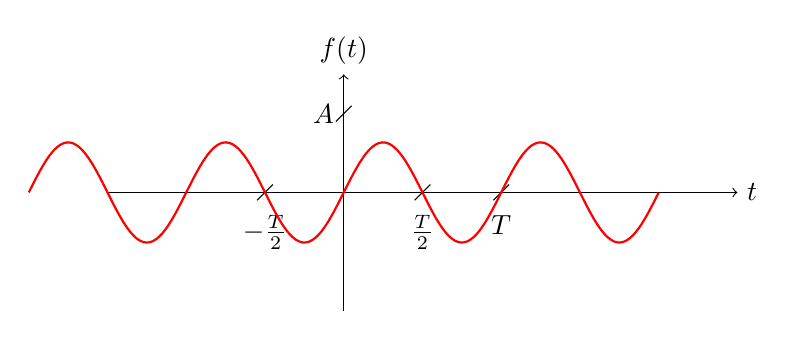
\begin{tikzpicture}
  %\draw (0,0) circle (1in);
  \draw[->] (-3.0,+0.0) -- (+5.0,+0.0) node[right] {$t$};
  \draw[->] (+0.0,-1.5) -- (+0.0,+1.5) node[above] {$f(t)$};
  %\draw[-,red, thick] (-2.5,+0.0) -- (+0.0,+0.0);
  %\draw[-] (-1.0-0.1,-0.1)--(-1.0+0.1,0.1) node[midway, below, outer sep=10pt,align=center] {$-\frac{T}{2}$};
  \draw[-] (-1.0-0.1,-0.1)--(-1.0+0.1,0.1) node[midway, below, outer sep=5pt,align=center] {$-\frac{T}{2}$};
  \draw[-] (+1.0-0.1,-0.1)--(+1.0+0.1,0.1) node[midway, below, outer sep=5pt] {$\frac{T}{2}$};
  \draw[-] (+2.0-0.1,-0.1)--(+2.0+0.1,0.1) node[midway, below, outer sep=5pt] {$T$};
  \draw[-] (-0.1,1.0-0.1)--(+0.1,1.0+0.1) node[midway, left] {$A$};
  
  \draw[scale=1.0,domain=-4:4.0,samples=100,smooth,variable=\x,red,thick] plot ({\x},{0.0+2.0/3.141592*sin(\x*180.0/3.141592*1*3.141592/1.0)});
  \end{tikzpicture}
\end{figure}

W przypadku sumowania do $k_{max}=2$ otrzymujemy 

\begin{figure}[H]
  \centering
  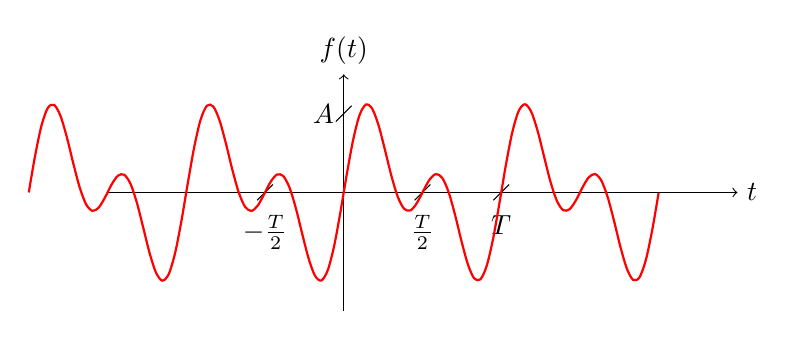
\begin{tikzpicture}
  %\draw (0,0) circle (1in);
  \draw[->] (-3.0,+0.0) -- (+5.0,+0.0) node[right] {$t$};
  \draw[->] (+0.0,-1.5) -- (+0.0,+1.5) node[above] {$f(t)$};
  %\draw[-,red, thick] (-2.5,+0.0) -- (+0.0,+0.0);
  %\draw[-] (-1.0-0.1,-0.1)--(-1.0+0.1,0.1) node[midway, below, outer sep=10pt,align=center] {$-\frac{T}{2}$};
  \draw[-] (-1.0-0.1,-0.1)--(-1.0+0.1,0.1) node[midway, below, outer sep=5pt,align=center] {$-\frac{T}{2}$};
  \draw[-] (+1.0-0.1,-0.1)--(+1.0+0.1,0.1) node[midway, below, outer sep=5pt] {$\frac{T}{2}$};
  \draw[-] (+2.0-0.1,-0.1)--(+2.0+0.1,0.1) node[midway, below, outer sep=5pt] {$T$};
  \draw[-] (-0.1,1.0-0.1)--(+0.1,1.0+0.1) node[midway, left] {$A$};
  
  \draw[scale=1.0,domain=-4:4.0,samples=100,smooth,variable=\x,red,thick] plot ({\x},{0.0+2.0/3.141592*sin(\x*180.0/3.141592*1*3.141592/1.0)+2.0/(3.141592)*sin(\x*180.0/3.141592*2*3.141592/1.0)});
  \end{tikzpicture}
\end{figure}

W przypadku sumowania do $k_{max}=3$ otrzymujemy 

\begin{figure}[H]
  \centering
  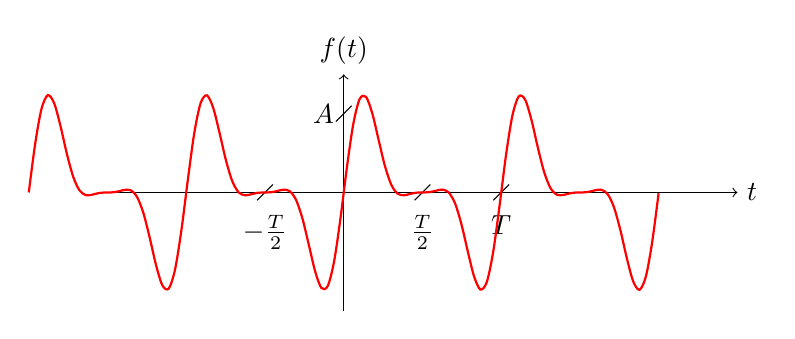
\begin{tikzpicture}
  %\draw (0,0) circle (1in);
  \draw[->] (-3.0,+0.0) -- (+5.0,+0.0) node[right] {$t$};
  \draw[->] (+0.0,-1.5) -- (+0.0,+1.5) node[above] {$f(t)$};
  %\draw[-,red, thick] (-2.5,+0.0) -- (+0.0,+0.0);
  %\draw[-] (-1.0-0.1,-0.1)--(-1.0+0.1,0.1) node[midway, below, outer sep=10pt,align=center] {$-\frac{T}{2}$};
  \draw[-] (-1.0-0.1,-0.1)--(-1.0+0.1,0.1) node[midway, below, outer sep=5pt,align=center] {$-\frac{T}{2}$};
  \draw[-] (+1.0-0.1,-0.1)--(+1.0+0.1,0.1) node[midway, below, outer sep=5pt] {$\frac{T}{2}$};
  \draw[-] (+2.0-0.1,-0.1)--(+2.0+0.1,0.1) node[midway, below, outer sep=5pt] {$T$};
  \draw[-] (-0.1,1.0-0.1)--(+0.1,1.0+0.1) node[midway, left] {$A$};
  
  \draw[scale=1.0,domain=-4:4.0,samples=100,smooth,variable=\x,red,thick] plot ({\x},{0.0+2.0/3.141592*sin(\x*180.0/3.141592*1*3.141592/1.0)+2.0/(1*3.141592)*sin(\x*180.0/3.141592*2*3.141592/1.0)+2.0/(3*3.141592)*sin(\x*180.0/3.141592*3*3.141592/1.0)});
  \end{tikzpicture}
\end{figure}

W przypadku sumowania do $k_{max}=5$ otrzymujemy 

\begin{figure}[H]
  \centering
  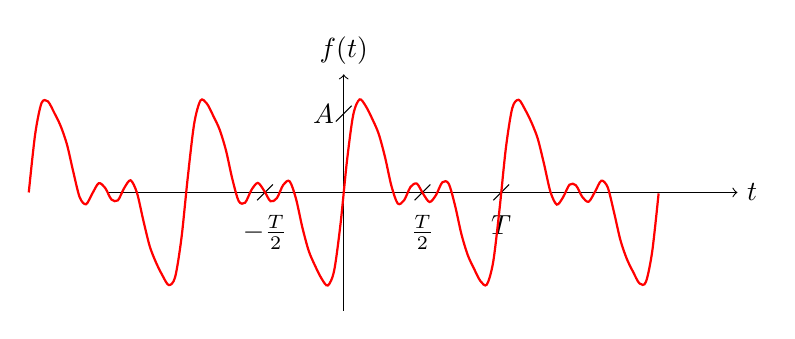
\begin{tikzpicture}
  %\draw (0,0) circle (1in);
  \draw[->] (-3.0,+0.0) -- (+5.0,+0.0) node[right] {$t$};
  \draw[->] (+0.0,-1.5) -- (+0.0,+1.5) node[above] {$f(t)$};
  %\draw[-,red, thick] (-2.5,+0.0) -- (+0.0,+0.0);
  %\draw[-] (-1.0-0.1,-0.1)--(-1.0+0.1,0.1) node[midway, below, outer sep=10pt,align=center] {$-\frac{T}{2}$};
  \draw[-] (-1.0-0.1,-0.1)--(-1.0+0.1,0.1) node[midway, below, outer sep=5pt,align=center] {$-\frac{T}{2}$};
  \draw[-] (+1.0-0.1,-0.1)--(+1.0+0.1,0.1) node[midway, below, outer sep=5pt] {$\frac{T}{2}$};
  \draw[-] (+2.0-0.1,-0.1)--(+2.0+0.1,0.1) node[midway, below, outer sep=5pt] {$T$};
  \draw[-] (-0.1,1.0-0.1)--(+0.1,1.0+0.1) node[midway, left] {$A$};
  
  \draw[scale=1.0,domain=-4:4.0,samples=100,smooth,variable=\x,red,thick] plot ({\x},{0.0+2.0/3.141592*sin(\x*180.0/3.141592*1*3.141592/1.0)+2.0/(1*3.141592)*sin(\x*180.0/3.141592*2*3.141592/1.0)+2.0/(3*3.141592)*sin(\x*180.0/3.141592*3*3.141592/1.0)+2.0/(5*3.141592)*sin(\x*180.0/3.141592*5*3.141592/1.0)});
  \end{tikzpicture}
\end{figure}

W przypadku sumowania do $k_{max}=6$ otrzymujemy 

\begin{figure}[H]
  \centering
  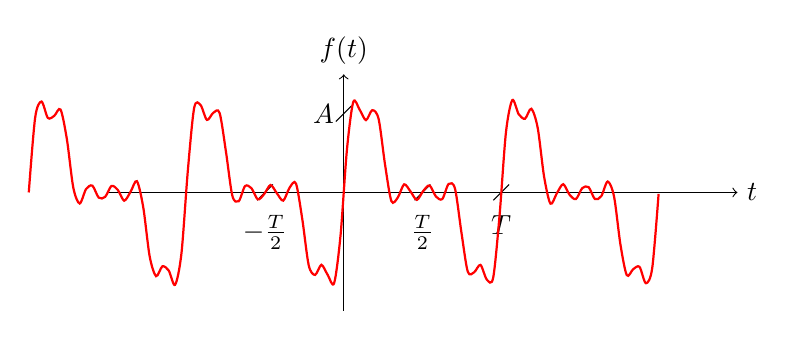
\begin{tikzpicture}
  %\draw (0,0) circle (1in);
  \draw[->] (-3.0,+0.0) -- (+5.0,+0.0) node[right] {$t$};
  \draw[->] (+0.0,-1.5) -- (+0.0,+1.5) node[above] {$f(t)$};
  %\draw[-,red, thick] (-2.5,+0.0) -- (+0.0,+0.0);
  %\draw[-] (-1.0-0.1,-0.1)--(-1.0+0.1,0.1) node[midway, below, outer sep=10pt,align=center] {$-\frac{T}{2}$};
  \draw[-] (-1.0-0.1,-0.1)--(-1.0+0.1,0.1) node[midway, below, outer sep=5pt,align=center] {$-\frac{T}{2}$};
  \draw[-] (+1.0-0.1,-0.1)--(+1.0+0.1,0.1) node[midway, below, outer sep=5pt] {$\frac{T}{2}$};
  \draw[-] (+2.0-0.1,-0.1)--(+2.0+0.1,0.1) node[midway, below, outer sep=5pt] {$T$};
  \draw[-] (-0.1,1.0-0.1)--(+0.1,1.0+0.1) node[midway, left] {$A$};
  
  \draw[scale=1.0,domain=-4:4.0,samples=100,smooth,variable=\x,red,thick] plot ({\x},{0.0+2.0/3.141592*sin(\x*180.0/3.141592*1*3.141592/1.0)+2.0/(1*3.141592)*sin(\x*180.0/3.141592*2*3.141592/1.0)+2.0/(3*3.141592)*sin(\x*180.0/3.141592*3*3.141592/1.0)+2.0/(5*3.141592)*sin(\x*180.0/3.141592*5*3.141592/1.0)+2.0/(3*3.141592)*sin(\x*180.0/3.141592*6*3.141592/1.0)});
  \end{tikzpicture}
\end{figure}

W przypadku sumowania do $k_{max}=11$ otrzymujemy 

\begin{figure}[H]
  \centering
  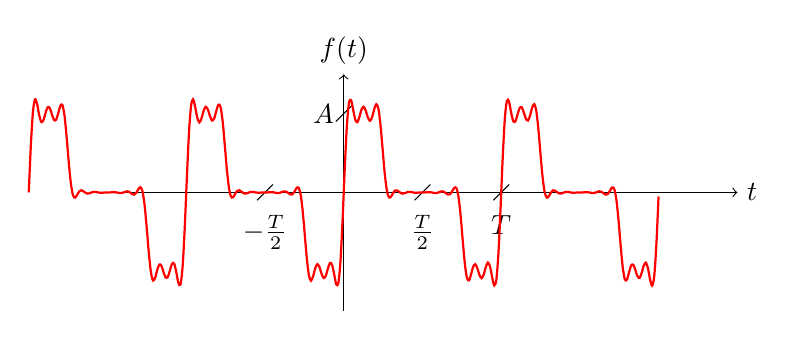
\begin{tikzpicture}
  %\draw (0,0) circle (1in);
  \draw[->] (-3.0,+0.0) -- (+5.0,+0.0) node[right] {$t$};
  \draw[->] (+0.0,-1.5) -- (+0.0,+1.5) node[above] {$f(t)$};
  %\draw[-,red, thick] (-2.5,+0.0) -- (+0.0,+0.0);
  %\draw[-] (-1.0-0.1,-0.1)--(-1.0+0.1,0.1) node[midway, below, outer sep=10pt,align=center] {$-\frac{T}{2}$};
  \draw[-] (-1.0-0.1,-0.1)--(-1.0+0.1,0.1) node[midway, below, outer sep=5pt,align=center] {$-\frac{T}{2}$};
  \draw[-] (+1.0-0.1,-0.1)--(+1.0+0.1,0.1) node[midway, below, outer sep=5pt] {$\frac{T}{2}$};
  \draw[-] (+2.0-0.1,-0.1)--(+2.0+0.1,0.1) node[midway, below, outer sep=5pt] {$T$};
  \draw[-] (-0.1,1.0-0.1)--(+0.1,1.0+0.1) node[midway, left] {$A$};
  
  \draw[scale=1.0,domain=-4:4.0,samples=300,smooth,variable=\x,red,thick] plot ({\x},{0.0+2.0/3.141592*sin(\x*180.0/3.141592*1*3.141592/1.0)+2.0/(1*3.141592)*sin(\x*180.0/3.141592*2*3.141592/1.0)+2.0/(3*3.141592)*sin(\x*180.0/3.141592*3*3.141592/1.0)+2.0/(5*3.141592)*sin(\x*180.0/3.141592*5*3.141592/1.0)+2.0/(3*3.141592)*sin(\x*180.0/3.141592*6*3.141592/1.0)+2.0/(7*3.141592)*sin(\x*180.0/3.141592*7*3.141592/1.0)+2.0/(9*3.141592)*sin(\x*180.0/3.141592*9*3.141592/1.0)+2.0/(5*3.141592)*sin(\x*180.0/3.141592*10*3.141592/1.0)+2.0/(11*3.141592)*sin(\x*180.0/3.141592*11*3.141592/1.0)});
  \end{tikzpicture}
\end{figure}

W przypadku sumowania do $k_{max}=21$ otrzymujemy 

\begin{figure}[H]
  \centering
  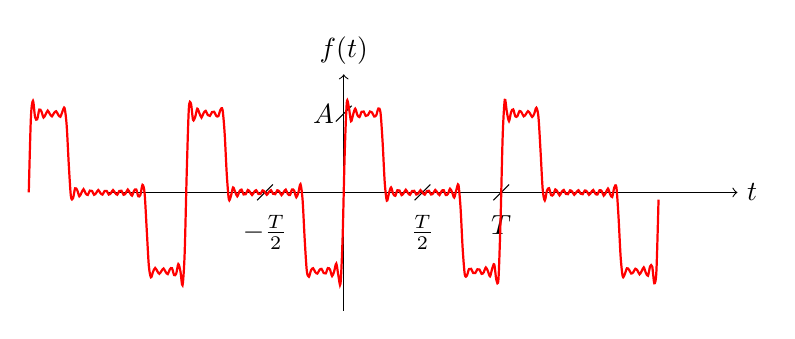
\begin{tikzpicture}
  %\draw (0,0) circle (1in);
  \draw[->] (-3.0,+0.0) -- (+5.0,+0.0) node[right] {$t$};
  \draw[->] (+0.0,-1.5) -- (+0.0,+1.5) node[above] {$f(t)$};
  %\draw[-,red, thick] (-2.5,+0.0) -- (+0.0,+0.0);
  %\draw[-] (-1.0-0.1,-0.1)--(-1.0+0.1,0.1) node[midway, below, outer sep=10pt,align=center] {$-\frac{T}{2}$};
  \draw[-] (-1.0-0.1,-0.1)--(-1.0+0.1,0.1) node[midway, below, outer sep=5pt,align=center] {$-\frac{T}{2}$};
  \draw[-] (+1.0-0.1,-0.1)--(+1.0+0.1,0.1) node[midway, below, outer sep=5pt] {$\frac{T}{2}$};
  \draw[-] (+2.0-0.1,-0.1)--(+2.0+0.1,0.1) node[midway, below, outer sep=5pt] {$T$};
  \draw[-] (-0.1,1.0-0.1)--(+0.1,1.0+0.1) node[midway, left] {$A$};
  
  \draw[scale=1.0,domain=-4:4.0,samples=300,smooth,variable=\x,red,thick] plot ({\x},{0.0+2.0/3.141592*sin(\x*180.0/3.141592*1*3.141592/1.0)+2.0/(1*3.141592)*sin(\x*180.0/3.141592*2*3.141592/1.0)+2.0/(3*3.141592)*sin(\x*180.0/3.141592*3*3.141592/1.0)+2.0/(5*3.141592)*sin(\x*180.0/3.141592*5*3.141592/1.0)+2.0/(3*3.141592)*sin(\x*180.0/3.141592*6*3.141592/1.0)+2.0/(7*3.141592)*sin(\x*180.0/3.141592*7*3.141592/1.0)+2.0/(9*3.141592)*sin(\x*180.0/3.141592*9*3.141592/1.0)+2.0/(5*3.141592)*sin(\x*180.0/3.141592*10*3.141592/1.0)+2.0/(11*3.141592)*sin(\x*180.0/3.141592*11*3.141592/1.0)+2.0/(13*3.141592)*sin(\x*180.0/3.141592*13*3.141592/1.0)+2.0/(7*3.141592)*sin(\x*180.0/3.141592*14*3.141592/1.0)+2.0/(15*3.141592)*sin(\x*180.0/3.141592*15*3.141592/1.0)+2.0/(17*3.141592)*sin(\x*180.0/3.141592*17*3.141592/1.0)+2.0/(9*3.141592)*sin(\x*180.0/3.141592*18*3.141592/1.0)+2.0/(19*3.141592)*sin(\x*180.0/3.141592*19*3.141592/1.0)+2.0/(21*3.141592)*sin(\x*180.0/3.141592*21*3.141592/1.0)});
  \end{tikzpicture}
\end{figure}

W granicy sumowania do $k_{max}=\infty$ otrzymujemy oryginalny sygnał.

\end{task}